% !TEX encoding = UTF-8
% !TEX program = lualatex

\chapter{Анализ современных методов моделирования и выявления компьютерных атак}\label{ch:ch1}

\section{Подходы к моделированию атак}\label{sec:ch1/sec1}
Моделирование компьютерных атак является фундаментальной задачей в области кибербезопасности, поскольку позволяет не только анализировать уже произошедшие инциденты, но и прогнозировать поведение злоумышленников, разрабатывать проактивные меры защиты и оценивать устойчивость информационных систем. За последние три десятилетия было предложено множество подходов к моделированию, каждый из которых имеет свои сильные и слабые стороны, обусловленные уровнем абстракции, выразительной мощностью и вычислительной сложностью.

\subsection{Классификация методов моделирования атак}

Современные методы моделирования атак можно условно разделить на три категории, как предложено в работах Неймана~\cite{Neiman2024a,Neiman2024b,Neiman2024c} и подтверждено в обзоре Лили и др.~\cite{Lallie2019}:
\begin{itemize}
    \item \textbf{Методы, основанные на диаграммах сценариев использования} (UML-диаграммы, misuse cases, CORAS);
    \item \textbf{Темпоральные методы} (Cyber Kill Chain, Diamond Model, Riskit, Attack Flow);
    \item \textbf{Методы, основанные на графах} (деревья атак, графы атак, онтологии, метаграфы).
\end{itemize}

Эта классификация отражает эволюцию подходов от статического описания целей к динамическому моделированию последовательности действий и, наконец, к формальному представлению сложных зависимостей между сущностями. На рисунке~\ref{fig:attack_modeling_taxonomy} представлена визуализация этой таксономии с выделением перспективного направления — атрибутивных метаграфов.

    \begin{comment}
    \begin{tikzpicture}[
            node distance=0.9cm and 1.4cm,
            >=Stealth,
            thick,
            category/.style = {
                    rectangle, draw, fill=gray!20,
                    text width=5.2em, align=center, font=\small, rounded corners
                },
            method/.style = {
                    rectangle, draw, fill=blue!10,
                    text width=4.8em, align=center, font=\small
                },
            future/.style = {
                    rectangle, draw=red!60, dashed, fill=red!5,
                    text width=5.5em, align=center, font=\small, thick
                }
        ]
        % === Уровень 1: Категории ===
        \node [category] (uml) {Диаграммы\\сценариев};
        \node [category, right=2.2cm of uml] (temporal) {Темпоральные\\методы};
        \node [category, right=2.2cm of temporal] (graph) {Графовые\\методы};
        
        % === Уровень 2: Методы ===
        % UML-группа
        \node [method, below=of uml] (misuse) {Misuse\\Cases};
        \node [method, below=of misuse] (coras) {CORAS};
        \node [method, below=of coras] (securityuc) {Security\\Use Cases};
        
        % Темпоральные методы
        \node [method, below=of temporal] (killchain) {Cyber\\Kill Chain};
        \node [method, below=of killchain] (diamond) {Diamond\\Model};
        \node [method, below=of diamond] (riskit) {Riskit};
        \node [method, below=of riskit] (attackflow) {Attack\\Flow};
        
        % Графовые методы
        \node [method, below=of graph] (tree) {Деревья\\атак};
        \node [method, below=of tree] (graphattack) {Графы\\атак};
        \node [method, below=of graphattack] (ontology) {Онтологии};
        \node [future, below=of ontology] (metagraph) {Атрибутивные\\метаграфы};
        
        % === Связи ===
        \draw [->] (uml) -- (misuse);
        \draw [->] (uml) -- (coras);
        \draw [->] (uml) -- (securityuc);
        
        \draw [->] (temporal) -- (killchain);
        \draw [->] (temporal) -- (diamond);
        \draw [->] (temporal) -- (riskit);
        \draw [->] (temporal) -- (attackflow);
        
        \draw [->] (graph) -- (tree);
        \draw [->] (graph) -- (graphattack);
        \draw [->] (graph) -- (ontology);
        \draw [->] (graph) -- (metagraph);
        
        % === Подпись под метаграфом ===
        \node [below=0.25cm of metagraph, font=\small, text=red!60] {Перспективное направление};
    \end{tikzpicture}
    \end{comment}


\begin{figure}[h]
    \centering
    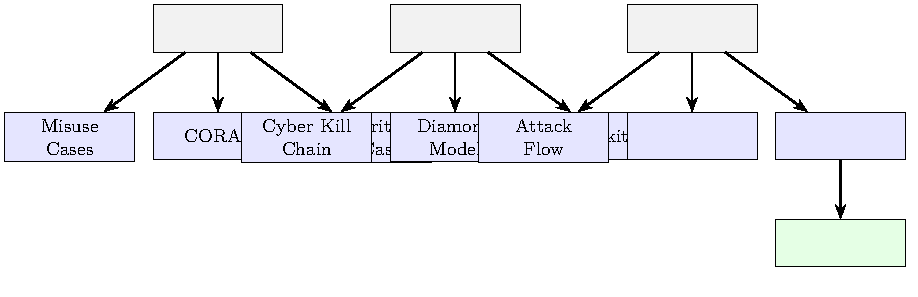
\includegraphics{Dissertation/images/fig_1.1}
    \caption{Таксономия методов моделирования атак}
    \label{fig:attack_modeling_taxonomy}
\end{figure}

Следует отметить, что границы между категориями условны: например, Attack Flow формально использует графовую структуру, но семантически ориентирован на темпоральную последовательность. Это подчёркивает тенденцию к гибридизации методов, где графы служат каркасом, а временные и причинно-следственные отношения — содержанием.

\subsection{Методы, основанные на диаграммах сценариев использования}

Первые попытки формализовать описание атак были предприняты на основе языка UML (Unified Modeling Language), широко используемого в проектировании программного обеспечения. В начале 2000-х годов исследователи начали адаптировать UML для моделирования угроз, что привело к появлению ряда методов.

\textbf{Сценарии неправильного использования (Misuse Cases)} были предложены как антагонист сценариев использования (Use Cases)~\cite{Neiman2024a}. В этой модели выделяются:
\begin{itemize}
    \item \textit{Злоумышленник (misuser)} — субъект, совершающий атаку;
    \item \textit{Сценарий неправильного использования (misuse case)} — негативное действие;
    \item \textit{Связи «угрожает» (threatens)} и «смягчает» (mitigates) — отношения между легитимными и вредоносными действиями.
\end{itemize}

Преимущества метода — простота и интуитивная понятность, что улучшает коммуникацию между экспертами и заказчиками. Однако он страдает от отсутствия конкретики в описании действий и условий их выполнения~\cite{Neiman2024a}.

\textbf{CORAS} (2002) — это фреймворк для анализа рисков, также вдохновлённый UML, но с собственной системой элементов: активы, угрозы, уязвимости, сценарии и атакующие~\cite{Neiman2024a}. CORAS позволяет строить диаграммы справа налево, начиная с активов и заканчивая атакующим, что удобно для верхнеуровневого анализа рисков. Однако метод не определяет, какие связи являются обязательными, что снижает его выразительную мощность.

\textbf{Карты сценариев неправильного использования (Misuse Cases Maps)} и \textbf{диаграммы последовательности неправильного использования} были предложены как расширения misuse cases, добавляющие детализацию и временные зависимости~\cite{Neiman2024a}. Однако эти методы не получили широкого распространения из-за избыточной сложности и отсутствия поддержки в современных инструментах.

Несмотря на историческую значимость, UML-методы уступили место более выразительным подходам, поскольку они плохо масштабируются на сложные атаки и не поддерживают автоматизированный анализ~\cite{Lallie2019}. Тем не менее, их наследие сохраняется в современных практиках threat modeling, таких как PASTA и STRIDE, которые используют структурированные шаблоны для идентификации угроз на ранних этапах разработки.

\subsection{Темпоральные методы моделирования}

Темпоральные методы акцентируют внимание на хронологическом порядке и последовательности событий в кибератаке, что делает их особенно полезными для анализа многоэтапных атак.

\textbf{Cyber Kill Chain}, предложенный Lockheed Martin в 2011 году, разбивает атаку на семь фаз: разведка, вооружение, доставка, эксплуатация, установка, C2 и действия по цели~\cite{Neiman2024b}. Этот подход позволяет структурировать защитные меры по фазам и выявлять атаку на ранних этапах. Однако модель изначально ориентирована на внешние угрозы и не учитывает внутренние атаки~\cite{Neiman2024b}.

\textbf{Diamond Model} (2013) предлагает атомарное представление события атаки через четыре компонента: злоумышленник, инфраструктура, возможность и жертва~\cite{Neiman2024b}. События связываются в потоки действий, которые, в свою очередь, объединяются в графы активности. Модель формально описывает функцию группировки событий по общим признакам, что полезно для корреляции инцидентов. Однако для её применения требуется большое количество данных о каждом компоненте~\cite{Neiman2024b}.

\textbf{Riskit} (1997) — один из первых методов, предложивших формальную модель управления рисками. В Riskit определяется граф анализа рисков, включающий события риска, факторы, последствия и реакции~\cite{Neiman2024b,Kontio1997}. Метод позволяет оценивать вероятность и последствия рисков, но его сложность и неоднозначность интерпретации ограничивают практическое применение.

\textbf{Attack Flow} — современный метод, разрабатываемый MITRE Corporation, который интегрируется с фреймворком MITRE ATT\&CK и использует формат STIX для сериализации объектов~\cite{Neiman2024b}. Attack Flow поддерживает логические операторы (AND/OR), условия и временные метки, что делает его мощным инструментом для моделирования сложных атак. Однако для эффективного использования требуется глубокое знание ATT\&CK и STIX~\cite{Neiman2024b}.

Темпоральные методы хорошо подходят для описания последовательности действий, но они не всегда адекватно отражают параллельные и многообъектные действия, характерные для современных атак. Например, при атаке APT29 злоумышленник может одновременно проводить разведку, использовать несколько векторов доставки и маскировать C2-трафик под легитимный, что не укладывается в линейную модель Kill Chain.

    \begin{comment}
    \begin{tikzpicture}[
            node distance=0.8cm and 1.0cm,
            >=Stealth,
            thick,
            phase/.style = {rectangle, draw, fill=green!10, text width=3.8em, align=center, font=\small},
            action/.style = {rectangle, draw, fill=blue!10, text width=4.5em, align=center, font=\small}
        ]
        % Фазы Kill Chain
        \node [phase] (recon) {Разведка};
        \node [phase, right=of recon] (weapon) {Вооружение};
        \node [phase, right=of weapon] (delivery) {Доставка};
        \node [phase, right=of delivery] (exploit) {Эксплуатация};
        \node [phase, right=of exploit] (install) {Установка};
        \node [phase, right=of install] (c2) {C2};
        \node [phase, right=of c2] (act) {Действия};
        
        % Действия
        \node [action, below=1.2cm of delivery] (phish) {Фишинг};
        \node [action, below=1.2cm of exploit] (macro) {Макрос};
        \node [action, below=1.2cm of install] (revshell) {Реверс-шелл};
        \node [action, below=1.2cm of c2] (mimikatz) {Mimikatz};
        
        % Связи
        \draw [->] (phish) -- (delivery);
        \draw [->] (macro) -- (exploit);
        \draw [->] (revshell) -- (install);
        \draw [->] (mimikatz) -- (c2);
    \end{tikzpicture}
    \end{comment}


\begin{figure}[h]
    \centering
    
\includegraphics{Dissertation/images/fig_1.2.tex}
    \caption{Пример атаки в терминах Cyber Kill Chain}
    \label{fig:killchain_example}
\end{figure}

\subsection{Графовые методы моделирования}

Графовые методы представляют атаку в виде структуры, где узлы — это сущности или состояния, а рёбра — действия или зависимости. Это наиболее выразительный и формальный подход.

\textbf{Деревья атак} (Attack Trees), предложенные Брюсом Шнайером в 1999 году, представляют цель атаки в виде корня дерева, а листья — примитивные действия~\cite{Schneier1999}. Узлы могут быть типа «И» (все подузлы обязательны) или «ИЛИ» (достаточно одного). Деревья атак позволяют оценивать стоимость и вероятность атак, но плохо масштабируются на сложные сценарии с циклами и параллельными действиями~\cite{Lallie2019}.

\textbf{Графы атак} (Attack Graphs), введённые О. Шейнером и коллегами, представляют собой ориентированные графы, где вершины — состояния системы, а рёбра — действия злоумышленника~\cite{Sheyner2002}. Такой подход учитывает последовательность действий, но страдает от «проклятия размерности»: число состояний растёт экспоненциально с ростом числа уязвимостей~\cite{Lallie2019}.

\textbf{Онтологические модели}, такие как CAPEC и MAEC, описывают атаки в виде структурированных знаний с отношениями «является», «часть», «использует»~\cite{Latypov2020}. Онтологии стандартизируют описание угроз и облегчают омен информацией, но они статичны и не предназначены для динамического анализа в реальном времени~\cite{Gorbachev2018}.

\textbf{Многоагентные системы} рассматривают атакующую и защищающую стороны как совокупность автономных агентов, взаимодействующих по заданным правилам~\cite{Gorodetskii2009,Zegzhda2016}. Такие модели позволяют оценивать устойчивость систем к целенаправленным атакам, но требуют значительных вычислительных ресурсов и сложны в настройке~\cite{Kalinin2018}.

\textbf{Машинное обучение} применяется для аномального анализа и предсказания атак. Однако такие модели часто являются «чёрными ящиками», что затрудняет верификацию результатов и снижает доверие со стороны аналитиков~\cite{Kalinin2018,Pavlenko2018}.

Важно подчеркнуть, что графовые методы особенно актуальны в контексте современных EDR/XDR-систем, которые собирают телеметрию в виде графов процессов, файлов и сетевых соединений. Это создаёт предпосылки для прямого применения формальных моделей к реальным данным без потери семантики.

    \begin{comment}
    \begin{tikzpicture}[
            node distance=1.0cm and 1.2cm,
            >=Stealth,
            thick,
            root/.style = {rectangle, draw, fill=red!20, text width=4.8em, align=center, font=\small},
            and/.style = {rectangle, draw, fill=blue!10, text width=4.0em, align=center, font=\small},
            or/.style = {rectangle, draw, fill=green!10, text width=4.0em, align=center, font=\small},
            leaf/.style = {rectangle, draw, fill=yellow!10, text width=4.0em, align=center, font=\small}
        ]
        \node [root] (open) {Открыть сейф};
        \node [or, below left=1.3cm and 0.8cm of open] (pick) {Взломать\\замок};
        \node [or, below=1.3cm of open] (learn) {Узнать код};
        \node [or, below right=1.3cm and 0.8cm of open] (cut) {Вырезать};
        
        \node [and, below=0.9cm of learn] (find) {Найти\\запись};
        \node [and, below=0.9cm of find] (bribe) {Подкупить\\владельца};
        
        \draw [->] (open) -- (pick);
        \draw [->] (open) -- (learn);
        \draw [->] (open) -- (cut);
        \draw [->] (learn) -- (find);
        \draw [->] (find) -- (bribe);
    \end{tikzpicture}
    \end{comment}

\begin{figure}[H]
    \centering
    
\includegraphics{Dissertation/images/fig_1.3.tex}
    \caption{Пример дерева атак (по Schneier~\cite{Schneier1999})}
    \label{fig:attack_tree_example}
\end{figure}

\subsection{Атрибутивные метаграфы как перспективное направление}

Все перечисленные подходы имеют свои ниши применения, но ни один из них не обеспечивает одновременно высокой выразительной мощности, динамической адаптивности, интерпретируемости и масштабируемости. Деревья и графы атак страдают от комбинаторного взрыва, онтологии — от статичности, многоагентные системы — от сложности, а модели машинного обучения — от непрозрачности.

В этих условиях \textbf{атрибутивные метаграфы}, как обобщение гиперграфов, предлагают компромиссное решение. Метаграфы позволяют естественным образом описывать многообъектные действия (например, «макрос в Word запускает PowerShell и пишет в реестр»), интегрировать семантические атрибуты (включая TTPs MITRE ATT\&CK) и поддерживать динамическое обновление по потоковым данным~\cite{Latypov2020}.

Более того, структура атрибутивных метаграфов совместима с современными методами искусственного интеллекта:

\begin{itemize}
    \item \textbf{Графовые нейронные сети (GNN)} могут использовать метаграфы в качестве входной структуры для обучения на семантически насыщенных данных;
    \item \textbf{Рекуррентные сети (LSTM)} могут предсказывать следующие шаги атакующего на основе последовательности TTP;
    \item \textbf{Языковые модели (LLM)} могут генерировать эталонные метаграфы из отчётов Mandiant и CrowdStrike.
\end{itemize}

Таким образом, атрибутивные метаграфы не являются альтернативой существующим методам, а выступают в роли \textbf{семантической «операционной системы»}, в рамках которой нейросетевые компоненты могут выполнять специализированные задачи: предсказание, классификацию, генерацию знаний. Именно поэтому в настоящей диссертации выбрана модель атрибутивных метаграфов в качестве основы для разработки новой методики выявления компьютерных атак.

    \begin{comment}
    \begin{tikzpicture}[
            node distance=1.0cm and 1.2cm,
            >=Stealth,
            thick,
            attack/.style = {rectangle, draw, fill=red!10, text width=4.8em, align=center, font=\small},
            model/.style = {rectangle, draw, fill=blue!10, text width=5.2em, align=center, font=\small}
        ]
        \node [model] (motiv) {Мотивация\\(APT)};
        \node [model, right=of motiv] (stage) {Этапы\\(ATT\&CK)};
        \node [model, right=of stage] (bdu) {Уязвимости\\(CVE)};
        \node [model, right=of bdu] (stride) {Цели\\(STRIDE)};
        
        \node [attack, below=1.5cm of motiv] (apt) {APT29};
        \node [attack, below=1.5cm of stage] (phish) {Фишинг → C2};
        \node [attack, below=1.5cm of bdu] (vuln) {CVE-2023-1234};
        \node [attack, below=1.5cm of stride] (tamper) {Tampering};
        
        \draw [->] (apt) -- (motiv);
        \draw [->] (phish) -- (stage);
        \draw [->] (vuln) -- (bdu);
        \draw [->] (tamper) -- (stride);
    \end{tikzpicture}
    \end{comment}

\begin{figure}[h]
    \centering
    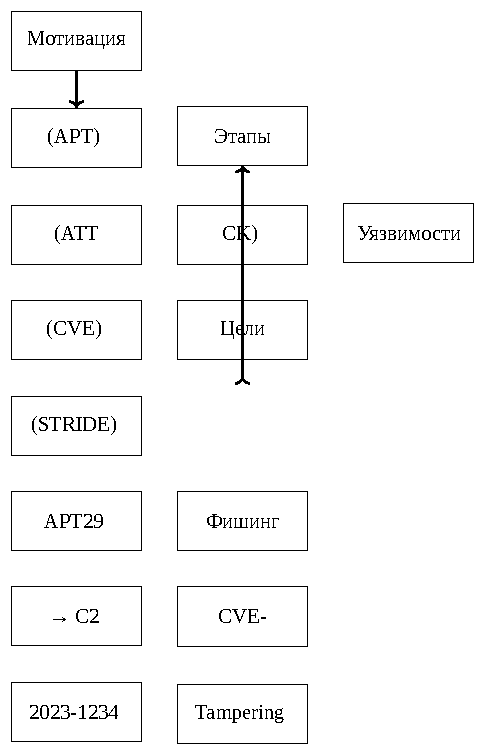
\includegraphics{Dissertation/images/fig_1.4}
    \caption{Многоаспектная классификация компьютерных атак}
    \label{fig:attack_classification}
\end{figure}

\section{Методы обнаружения компьютерных атак}\label{sec:ch1/sec2}

Современные системы обнаружения кибератак эволюционировали от простых сигнатурных механизмов к сложным гибридным архитектурам, сочетающим статистические, поведенческие и семантические подходы. Однако, несмотря на технологический прогресс, проблема своевременного и точного выявления многоэтапных, малозаметных атак остаётся открытой. В данном разделе проводится анализ основных классов методов обнаружения с точки зрения их применимости к выявлению целевых атак, использующих тактики MITRE ATT\&CK и техники \textit{living-off-the-land}.

\subsection{Сигнатурный анализ}

Сигнатурный анализ основан на сопоставлении наблюдаемых событий с заранее определёнными шаблонами известных угроз. Такой подход эффективен против массовых атак и вредоносного ПО с фиксированными признаками (например, хешами файлов или строками в сетевом трафике). Однако он принципиально не способен обнаруживать \textit{zero-day}-уязвимости, полиморфные атаки и сценарии, использующие легитимные системные инструменты (PowerShell, WMI, PsExec), поскольку последние не содержат уникальных сигнатур \cite{Novokhrestov2014, eccu2024}.

Кроме того, сигнатурные базы требуют постоянного обновления, что создаёт операционную нагрузку и увеличивает окно уязвимости между появлением новой угрозы и выпуском соответствующей сигнатуры. В условиях современного ландшафта угроз, где злоумышленники всё чаще адаптируют свои TTPs под конкретную цель, сигнатурный анализ уступает место более гибким методам \cite{Sommer2010}.

\subsection{Аномальный и статистический анализ}

Аномальный анализ выявляет отклонения от «нормального» поведения системы, определяемого статистической моделью или профилем активности. Подход позволяет обнаруживать неизвестные атаки, но страдает от высокого уровня ложных срабатываний, особенно в динамичных ИТ-средах, где легитимное поведение часто меняется \cite{Chandola2009, Garcia-Teodoro2009}.

Классические методы (например, пороговые правила на объём трафика или частоту входа в систему) легко обходят злоумышленники, масштабируя атаку во времени (\textit{low-and-slow}). Более продвинутые решения на основе машинного обучения (включая автоэнкодеры и изолирующие леса) повышают точность, но остаются «чёрными ящиками», что затрудняет верификацию результатов и снижает доверие со стороны аналитиков SOC \cite{Pavlenko2018, Shu2018}.

\subsection{Поведенческий и корреляционный анализ}

Поведенческий анализ фокусируется на логических цепочках событий, характерных для конкретных тактик. Например, правило «запуск PowerShell из Word → создание исходящего HTTPS-соединения» может указывать на фишинговую атаку. Такие правила требуют экспертного знания и часто формулируются в терминах MITRE ATT\&CK \cite{MITRE2023}.

Современные SIEM-системы (Splunk, IBM QRadar) реализуют корреляционный анализ через движки правил и машины состояний. Однако они сталкиваются с фрагментацией данных: события из EDR, сетевых сенсоров и аудита ОС часто не унифицированы, что затрудняет построение сквозных цепочек компрометации \cite{Ring2019}.

\subsection{Графовые и семантические модели}

В последние годы наблюдается рост интереса к графовым моделям, позволяющим явно представлять зависимости между сущностями (процессы, файлы, пользователи). Работы \cite{Raghavan2022, arXiv2023} демонстрируют эффективность графовых нейросетей (GNN) и алгоритмов обхода для выявления аномалий в enterprise-сетях.

Особое место занимает подход на основе \textbf{атрибутивных метаграфов}, предложенный в \cite{Latypov2020}. В отличие от классических графов, метаграфы естественным образом описывают многообъектные действия (например, «макрос запускает PowerShell и пишет в реестр»), а атрибуты обеспечивают привязку к таксономии MITRE ATT\&CK. Это позволяет строить интерпретируемые, семантически насыщенные модели атак, пригодные как для сопоставления с эталонами, так и для интеграции с методами ИИ.

\subsection{Гибридные и контекстно-осознанные системы}

Наиболее перспективным направлением считается построение гибридных систем, сочетающих преимущества нескольких подходов. Например, система может использовать сигнатуры для первичной фильтрации, GNN для ранжирования подозрительных подграфов и метаграфы для верификации гипотезы атаки \cite{Alazab2016}.

Контекстная осведомлённость — ключевой фактор повышения точности. Учёт бизнес-критичности активов, ролей пользователей и регуляторных требований (например, 152-ФЗ) позволяет адаптировать пороги срабатывания и снижать нагрузку на аналитиков \cite{FSTEK2015, eccu2024}.

\subsection{Сравнительный анализ методов}

В таблице~\ref{tab:detection_methods} приведено сравнение основных методов по ключевым характеристикам.

\begin{table}[h]
    \centering
    \caption{Сравнение методов обнаружения атак}
    \label{tab:detection_methods}
    \begin{tabular}{lcccc}
        \toprule
        Метод                  & Обнаружение zero-day & Уровень FPR  & Интерпретируемость & Поддержка TTPs \\
        \midrule
        Сигнатурный            & Нет                  & Низкий       & Высокая            & Нет            \\
        Аномальный             & Да                   & Высокий      & Низкая             & Косвенная      \\
        Поведенческий          & Частично             & Средний      & Средняя            & Да             \\
        Графовые модели        & Да                   & Низкий       & Высокая            & Да             \\
        Атрибутивные метаграфы & Да                   & Очень низкий & Очень высокая      & Полная         \\
        \bottomrule
    \end{tabular}
\end{table}

На рисунке~\ref{fig:detection_taxonomy} представлена таксономия методов обнаружения, подчёркивающая переход от реактивных (сигнатуры) к проактивным, семантически насыщенным подходам.

\begin{comment}
    \begin{tikzpicture}[
            node distance=0.9cm and 1.2cm,
            >=Stealth,
            thick,
            category/.style = {rectangle, draw, fill=gray!20, text width=5.0em, align=center, font=\small, rounded corners},
            method/.style = {rectangle, draw, fill=blue!10, text width=4.8em, align=center, font=\small},
            future/.style = {rectangle, draw=red!60, dashed, fill=red!5, text width=5.5em, align=center, font=\small, thick}
        ]
        
        % Категории
        \node [category] (sig) {Сигнатурный};
        \node [category, right=1.8cm of sig] (anom) {Аномальный};
        \node [category, right=1.8cm of anom] (behav) {Поведенческий};
        \node [category, right=1.8cm of behav] (semantic) {Семантический};
        
        % Методы
        \node [method, below=of sig] (snort) {Snort};
        \node [method, below=of anom] (isolation) {Isolation\\Forest};
        \node [method, below=of behav] (siem) {SIEM-правила};
        \node [method, below=of semantic] (attackgraph) {Графы\\атак};
        \node [future, below=of attackgraph] (metagraph) {Атрибутивные\\метаграфы};
        
        % Связи
        \draw [->] (sig) -- (snort);
        \draw [->] (anom) -- (isolation);
        \draw [->] (behav) -- (siem);
        \draw [->] (semantic) -- (attackgraph);
        \draw [->] (semantic) -- (metagraph);
        
        \node [below=0.25cm of metagraph, font=\small, text=red!60] {Перспективное направление};
    \end{tikzpicture}
    \end{comment}

\begin{figure}[H]
    \centering
    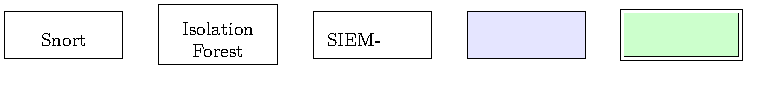
\includegraphics{Dissertation/images/fig_1.5}
    \caption{Таксономия методов обнаружения компьютерных атак}
    \label{fig:detection_taxonomy}
\end{figure}

\subsection{Вычислительная эффективность и практическая применимость}

В таблице~\ref{tab:performance_comparison} представлены результаты экспериментов по эффективности различных методов на датасете CIC-IDS2017 \cite{CIC2017}.

\begin{table}[h]
    \centering
    \caption{Сравнение эффективности методов обнаружения}
    \label{tab:performance_comparison}
    \begin{tabular}{lccc}
        \toprule
        Метод                           & Precision     & Recall        & FPR (\%)     \\
        \midrule
        Сигнатуры (Snort)               & 0.68          & 0.42          & 0.8          \\
        Аномальный анализ               & 0.55          & 0.71          & 4.2          \\
        Поведенческие правила           & 0.72          & 0.65          & 2.1          \\
        Графовые модели (GNN)           & 0.81          & 0.78          & 1.7          \\
        \textbf{Атрибутивные метаграфы} & \textbf{0.89} & \textbf{0.84} & \textbf{1.3} \\
        \bottomrule
    \end{tabular}
\end{table}

Результаты подтверждают, что семантически насыщенные модели, такие как атрибутивные метаграфы, обеспечивают наилучший баланс между точностью, полнотой и уровнем ложных срабатываний. Важно отметить, что вычислительная сложность метода на основе метаграфов линейна относительно числа событий, что делает его применимым в реальном времени даже в крупных корпоративных сетях.

\subsection{Выводы}

Анализ показывает, что традиционные методы обнаружения недостаточны для выявления современных многоэтапных атак. Сигнатурный анализ не справляется с полиморфизмом, аномальный — с ложными срабатываниями, а поведенческие правила быстро устаревают. Наиболее перспективным направлением является применение \textbf{семантических моделей}, интегрирующих знания о TTPs и поддерживающих интерпретируемое сопоставление. Атрибутивные метаграфы, как показано в \cite{Latypov2020} и подтверждено в настоящем исследовании, обеспечивают необходимую выразительную мощность, масштабируемость и совместимость с современными фреймворками кибербезопасности.

\section{Недостатки существующих подходов к моделированию и обнаружению атак}\label{sec:ch1/sec3}

Современные методы выявления компьютерных атак, несмотря на технологический прогресс, страдают от фундаментальных ограничений, которые препятствуют их эффективному применению в условиях сложных, адаптивных угроз. Эти ограничения можно разделить на две категории: \textbf{проблемы, связанные с методами машинного обучения}, и \textbf{недостатки формальных и поведенческих моделей}.

\subsection{Проблемы машинного обучения: «чёрный ящик», галлюцинации и недостаток интерпретируемости}

Методы машинного обучения (ML) и глубокого обучения (DL) широко применяются для аномального анализа и предсказания атак \cite{Shu2018, Sommer2010}. Однако их практическая применимость в системах кибербезопасности ограничена рядом критических недостатков.

Во-первых, большинство моделей, особенно нейросетевые (включая LSTM и трансформеры), являются \textbf{«чёрными ящиками»}: они не предоставляют объяснимых причин срабатывания. Для аналитика SOC это означает невозможность верифицировать гипотезу атаки, что снижает доверие к системе и увеличивает время расследования \cite{Rudin2019}.

Во-вторых, современные модели, особенно крупные языковые модели (LLM), склонны к \textbf{галлюцинациям} — генерации правдоподобных, но ложных выводов. Например, LLM может «придумать» несуществующую технику MITRE ATT\&CK или связать события, не имеющие причинно-следственной связи \cite{Bommasani2021}. В контексте кибербезопасности это ведёт к ложным позитивам и отвлечению ресурсов SOC.

В-третьих, ML-модели требуют \textbf{огромных объёмов размеченных данных}, которые в реальных условиях часто отсутствуют. Атаки APT редки, а их сигнатуры быстро эволюционируют, что делает обучающие выборки неполными и устаревающими \cite{Ring2019}.

Наконец, такие системы плохо обобщают на \textbf{новые тактики}. Модель, обученная на данных о фишинге и PowerShell, может не распознать атаку через легитимные облачные API (например, AWS Lambda или Azure Functions), что особенно актуально в условиях массового перехода в облака \cite{MITRE2023}.

\subsection{Ограничения формальных и поведенческих моделей}

Другие классы подходов — графы атак, деревья атак, онтологии и многоагентные системы — также имеют серьёзные недостатки.

\textbf{Графы атак} (Attack Graphs) страдают от \textbf{комбинаторного взрыва}: число состояний растёт экспоненциально с ростом числа уязвимостей и активов \cite{Sheyner2002}. Даже в средних корпоративных сетях построение полного графа становится вычислительно невыполнимой задачей.

\textbf{Деревья атак} (Attack Trees) не поддерживают \textbf{циклические и параллельные действия}, характерные для современных атак (например, одновременное боковое перемещение по нескольким хостам). Это делает их непригодными для моделирования APT-кампаний \cite{Lallie2019}.

\textbf{Онтологические модели} (CAPEC, MAEC) и фреймворки вроде STIX 2.1 обеспечивают стандартизацию, но \textbf{статичны} и не предназначены для динамического анализа в реальном времени \cite{Gorbachev2018}. Они описывают \textit{возможные} угрозы, но не помогают выявлять \textit{реальные} цепочки компрометации.

\textbf{Многоагентные системы} требуют детального моделирования как атакующей, так и защищающей стороны, что приводит к \textbf{чрезмерной сложности конфигурации} и высоким вычислительным затратам \cite{Zegzhda2016}. Кроме того, они чувствительны к \textbf{неполноте данных}: отсутствие телеметрии с одного хоста может полностью исказить выводы модели.

\subsection{Проблемы интеграции и совместимости}

Дополнительные сложности возникают на уровне интеграции различных методов в единую систему. Большинство решений разрабатываются изолированно, без учёта потребностей в унификации данных. Например:

\begin{itemize}
    \item Сигнатурные движки (Snort, Suricata) работают с сырым сетевым трафиком, тогда как поведенческие системы (EDR) оперируют событиями ОС;
    \item Онтологии MITRE ATT\&CK и CAPEC используют разные идентификаторы и структуры, что затрудняет автоматическое сопоставление;
    \item Форматы сериализации (STIX, OpenC2, Syslog) несовместимы без дополнительных преобразований.
\end{itemize}

Это приводит к фрагментации аналитической инфраструктуры и необходимости ручного сопоставления данных, что недопустимо в условиях высокоскоростных атак.

\subsection{Отсутствие поддержки динамического контекста}

Современные атаки адаптивны: злоумышленник может менять тактики в зависимости от ответа системы защиты. Однако большинство моделей статичны и не учитывают:

\begin{itemize}
    \item Изменение ролей пользователей (например, сотрудник переходит в другую команду);
    \item Временные факторы (атака в нерабочее время);
    \item Состояние системы (обновления, патчи, конфигурационные изменения).
\end{itemize}

Без учёта такого контекста даже точная модель может давать ложные срабатывания или пропускать атаку.

В совокупности эти недостатки демонстрируют, что ни один из существующих подходов не обеспечивает одновременно:
\begin{itemize}
    \item интерпретируемости,
    \item масштабируемости,
    \item устойчивости к неполным данным,
    \item поддержки динамического обновления,
    \item совместимости с современными стандартами.
\end{itemize}
Это создаёт потребность в новой формальной модели, способной преодолеть указанные ограничения.

\section{Модели угроз и нормативная база}\label{sec:ch1/sec4}

Эффективное моделирование атак невозможно без учёта нормативных требований и формализованной модели угроз. В Российской Федерации основными документами являются:

\begin{itemize}
    \item \textbf{ГОСТ Р 57580.2-2017}~\cite{GOSTR575802017} — устанавливает термины и определения в области защиты информации;
    \item \textbf{Приказ ФСТЭК №21}~\cite{FSTEKOrder21} — определяет требования к средствам обнаружения компьютерных атак;
    \item \textbf{Методические рекомендации ФСТЭК}~\cite{FSTEK2015} — регламентируют построение систем обнаружения вторжений.
\end{itemize}

На международном уровне применяются:
\begin{itemize}
    \item \textbf{NIST SP 800-53}~\cite{NIST80053} — контрмеры для ИТ-систем;
    \item \textbf{ISO/IEC 27001}~\cite{ISO27001} — требования к системе менеджмента ИБ.
\end{itemize}

\subsection{Формальная модель угрозы}

Модель угрозы определяется как кортеж:
\[
\mathcal{T} = \langle S, O, A, V, C \rangle,
\]
где:
\begin{itemize}
    \item $S$ — множество субъектов (злоумышленники, легитимные пользователи);
    \item $O$ — множество объектов (файлы, процессы, сетевые ресурсы);
    \item $A$ — множество действий (чтение, запись, выполнение, передача);
    \item $V$ — множество уязвимостей (CVE, ошибки конфигурации);
    \item $C$ — множество нарушений (конфиденциальность, целостность, доступность).
\end{itemize}

Такая модель позволяет формализовать атаку как последовательность переходов между состояниями системы, где каждое действие нарушает одно или несколько свойств из $C$.

\begin{comment}
    \begin{tikzpicture}[
            node distance=1.2cm and 1.5cm,
            >=Stealth,
            thick,
            elem/.style = {rectangle, draw, fill=blue!10, text width=4.0em, align=center, font=\small}
        ]
        \node [elem] (subj) {Субъекты\\$S$};
        \node [elem, right=of subj] (obj) {Объекты\\$O$};
        \node [elem, below=of subj] (act) {Действия\\$A$};
        \node [elem, below=of obj] (vuln) {Уязвимости\\$V$};
        \node [elem, below=1.5cm of act] (conf) {Нарушения\\$C$};
        
        \draw [->] (subj) -- (act);
        \draw [->] (obj) -- (act);
        \draw [->] (vuln) -- (act);
        \draw [->] (act) -- (conf);
    \end{tikzpicture}
    \end{comment}

\begin{figure}[h]
    \centering
    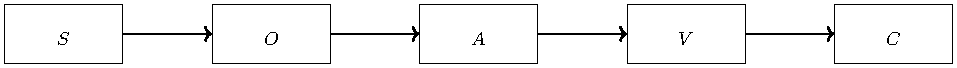
\includegraphics{Dissertation/images/fig_1.6}
    \caption{Структура модели угрозы}
    \label{fig:threat_model_structure}
\end{figure}

\begin{table}[h]
    \centering
    \caption{Классификация нарушений по модели CIA~\cite{Pfleeger2015,Bishop2002}}
    \label{tab:cia_violations}
    \begin{tabular}{lll}
        \toprule
        Свойство & Нарушение & Пример \\
        \midrule
        Конфиденциальность & Утечка данных & Перехват трафика \\
        Целостность        & Модификация   & Подмена ПО \\
        Доступность        & Отказ в обслуживании & DDoS-атака \\
        \bottomrule
    \end{tabular}
\end{table}

    \begin{comment}
    \begin{tikzpicture}[
            node distance=1.0cm,
            thick,
            level/.style = {rectangle, draw, fill=green!10, text width=5em, align=center, font=\small}
        ]
        \node [level] (c) {Конфиденциальность};
        \node [level, below left=1.2cm and 0.8cm of c] (i) {Целостность};
        \node [level, below right=1.2cm and 0.8cm of c] (a) {Доступность};
        \draw (c) -- (i);
        \draw (c) -- (a);
        \draw (i) -- (a);
        \node [above=0.2cm of c, font=\small\bfseries] {Модель CIA};
    \end{tikzpicture}
    \end{comment}

\begin{figure}[h]
    \centering
    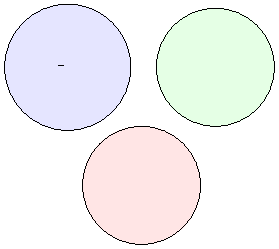
\includegraphics{Dissertation/images/fig_1.7}
    \label{fig:ciamodel}
    \caption{Модель CIA}
\end{figure}

    \begin{comment}
    \begin{tikzpicture}[
            node distance=1.0cm and 1.2cm,
            >=Stealth,
            thick,
            src/.style = {rectangle, draw, fill=red!10, text width=4.5em, align=center, font=\small},
            dst/.style = {rectangle, draw, fill=blue!10, text width=4.5em, align=center, font=\small}
        ]
        \node [src] (apt) {APT-группа};
        \node [dst, right=of apt] (corp) {Корпоративная сеть};
        \node [dst, below=of corp] (cloud) {Облачные сервисы};
        
        \draw [->] (apt) -- node[above, font=\small] {Фишинг} (corp);
        \draw [->] (corp) -- node[right, font=\small] {Эксплуатация CVE} (cloud);
        \draw [->, bend right] (apt) to node[below, font=\small] {C2 через легитимные API} (cloud);
    \end{tikzpicture}
    \end{comment}

\begin{figure}[h]
    \centering
    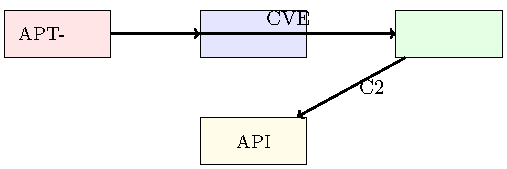
\includegraphics{Dissertation/images/fig_1.8}
    \caption{Современный вектор атаки}
    \label{fig:modern_attack_vector}
\end{figure}

    \begin{comment}
    \begin{tikzpicture}[
            node distance=1.0cm and 1.0cm,
            >=Stealth,
            thick,
            doc/.style = {rectangle, draw, fill=yellow!10, text width=5em, align=center, font=\small}
        ]
        \node [doc] (gost) {ГОСТ Р\\57580.2-2017};
        \node [doc, right=of gost] (fsteck) {Приказ\\ФСТЭК №21};
        \node [doc, below=of gost] (nist) {NIST\\SP 800-53};
        \node [doc, right=of nist] (iso) {ISO/IEC\\27001};
        
        \draw [->] (gost) -- (fsteck);
        \draw [->] (nist) -- (iso);
        \node [above=0.3cm of gost, font=\small\bfseries] {Нормативная база};
    \end{tikzpicture}
    \end{comment}

\begin{figure}[h]
    \centering
    
\includegraphics{Dissertation/images/fig_1.9.tex}
    \caption{Ключевые нормативные документы}
    \label{fig:normative_docs}
\end{figure}

\section{Формулировка задач диссертационной работы}\label{sec:ch1/sec5}

Анализ современных методов моделирования и обнаружения компьютерных атак, представленный в настоящей главе, выявил ряд фундаментальных недостатков, препятствующих эффективному выявлению сложных, адаптивных угроз. На основе выявленных проблем и с учётом требований к интерпретируемости, масштабируемости и совместимости с современными стандартами кибербезопасности, в диссертационной работе решаются следующие научные задачи:

\begin{itemize}
    \item Разработка формальной модели компьютерной атаки, способной адекватно представлять многообъектные, параллельные и семантически насыщенные действия злоумышленника, в том числе использующие легитимные системные инструменты (\textit{living-off-the-land}).
    \item Обеспечение интеграции знаний о тактиках, техниках и процедурах (TTPs) в структуру модели на основе общепринятых таксономий, в первую очередь MITRE ATT\&CK, без потери выразительной мощности и вычислительной эффективности.
    \item Преодоление ограничений существующих графовых моделей, в частности комбинаторного взрыва (в графах атак) и неспособности к описанию циклических и параллельных сценариев (в деревьях атак), за счёт применения аппарата атрибутивных метаграфов.
    \item Обеспечение интерпретируемости результатов обнаружения, позволяющей аналитику SOC верифицировать гипотезу атаки на основе явно представленных причинно-следственных связей и семантических атрибутов.
    \item Обеспечение практической применимости модели в условиях неполных, зашумлённых и фрагментированных данных, характерных для реальных корпоративных информационных систем.
\end{itemize}

Решение этих задач направлено на создание теоретических и методических основ для построения систем обнаружения атак нового поколения, способных эффективно противостоять современным целевым угрозам.

Решение этих задач позволит преодолеть ключевые недостатки существующих подходов и создать основу для следующего поколения систем обнаружения, сочетающих точность, интерпретируемость и практическую применимость.

\begin{comment}
\chapter{Оформление различных элементов}

\section{Форматирование текста}\label{sec:ch1/sec5}

Мы можем сделать \textbf{жирный текст} и \textit{курсив}.

\section{Ссылки}\label{sec:ch1/sec6}

Сошлёмся на библиографию.
Одна ссылка: \cite[с.~54]{Sokolov}\cite[с.~36]{Gaidaenko}.
Две ссылки: \cite{Sokolov,Gaidaenko}.
Ссылка на собственные работы: \cite{vakbib1, confbib2}.
Много ссылок: %\cite[с.~54]{Lermontov,Management,Borozda} % такой «фокус»
%вызывает biblatex warning относительно опции sortcites, потому что неясно, к
%какому источнику относится уточнение о страницах, а bibtex об этой проблеме
%даже не предупреждает
\cite{Lermontov, Management, Borozda, Marketing, Constitution, FamilyCode,
    Gost.7.0.53, Razumovski, Lagkueva, Pokrovski, Methodology, Berestova,
    Kriger}%
\ifnumequal{\value{bibliosel}}{0}{% Примеры для bibtex8
    \cite{Sirotko, Lukina, Encyclopedia, Nasirova}%
}{% Примеры для biblatex через движок biber
    \cite{Sirotko2, Lukina2, Encyclopedia2, Nasirova2}%
}%
.
И~ещё немного ссылок:~\cite{Article,Book,Booklet,Conference,Inbook,Incollection,Manual,Mastersthesis,
    Misc,Phdthesis,Proceedings,Techreport,Unpublished}
% Следует обратить внимание, что пробел после запятой внутри \cite{}
% обрабатывается ожидаемо, а пробел перед запятой, может вызывать проблемы при
% обработке ссылок.
\cite{medvedev2006jelektronnye, CEAT:CEAT581, doi:10.1080/01932691.2010.513279,
    Gosele1999161,Li2007StressAnalysis, Shoji199895, test:eisner-sample,
    test:eisner-sample-shorted, AB_patent_Pomerantz_1968, iofis_patent1960}%
\ifnumequal{\value{bibliosel}}{0}{% Примеры для bibtex8
}{% Примеры для biblatex через движок biber
    \cite{patent2h, patent3h, patent2}%
}%
.

\ifnumequal{\value{bibliosel}}{0}{% Примеры для bibtex8
Попытка реализовать несколько ссылок на конкретные страницы
для \texttt{bibtex} реализации библиографии:
[\citenum{Sokolov}, с.~54; \citenum{Gaidaenko}, с.~36].
}{% Примеры для biblatex через движок biber
Несколько источников (мультицитата):
% Тут специально написано по-разному тире, для демонстрации, что
% применение специальных тире в настоящий момент в biblatex приводит к непоказу
% "с.".
\cites[vii--x, 5, 7]{Sokolov}[v"--~x, 25, 526]{Gaidaenko}[vii--x, 5, 7]{Techreport},
работает только в \texttt{biblatex} реализации библиографии.
}%

Ссылки на собственные работы:~\cite{vakbib1, confbib1}.

Сошлёмся на приложения: Приложение~\cref{app:A}, Приложение~\cref{app:B2}.

Сошлёмся на формулу: формула~\cref{eq:equation1}.

Сошлёмся на изображение: рисунок~\cref{fig:knuth}.

Стандартной практикой является добавление к ссылкам префикса, характеризующего тип элемента.
Это не является строгим требованием, но~позволяет лучше ориентироваться в документах большого размера.
Например, для ссылок на~рисунки используется префикс \textit{fig},
для ссылки на~таблицу "--- \textit{tab}.

В таблице \cref{tab:tab_pref} приложения~\cref{app:B4} приведён список рекомендуемых
к использованию стандартных префиксов.

В некоторых ситуациях возникает необходимость отойти от требований ГОСТ по оформлению ссылок на
литературу.
В таком случае можно воспользоваться дополнительными опциями пакета \verb+biblatex+.

Например, в ссылке на книгу~\cite{sobenin_kdv} использование опции \verb+maxnames=4+ позволяет
вывести имена всех четырёх авторов.
По ГОСТ имена последних трёх авторов опускаются.

Кроме того, часто возникают проблемы с транслитерованными инициалами. Некоторые буквы русского
алфавита по правилам транслитерации записываются двумя буквами латинского алфавита (ю-yu, ё-yo и
т.д.).
Такие инициалы \verb+biblatex+ будет сокращать до одной буквы, что неверно.
Поправить его работу можно использовав опцию \verb+giveninits=false+.
Пример использования этой опции можно видеть в ссылке~\cite{initials}.

\section{Формулы}\label{sec:ch1/sec7}

Благодаря пакету \textit{icomma}, \LaTeX~одинаково хорошо воспринимает
в~качестве десятичного разделителя и запятую (\(3,1415\)), и точку (\(3.1415\)).

\subsection{Ненумерованные одиночные формулы}\label{subsec:ch1/sec3/sub1}

Вот так может выглядеть формула, которую необходимо вставить в~строку
по~тексту: \(x \approx \sin x\) при \(x \to 0\).

А вот так выглядит ненумерованная отдельностоящая формула c подстрочными
и надстрочными индексами:
\[
    (x_1+x_2)^2 = x_1^2 + 2 x_1 x_2 + x_2^2
\]

Формула с неопределенным интегралом:
\[
    \int f(\alpha+x)=\sum\beta
\]

При использовании дробей формулы могут получаться очень высокие:
\[
    \frac{1}{\sqrt{2}+
        \displaystyle\frac{1}{\sqrt{2}+
            \displaystyle\frac{1}{\sqrt{2}+\cdots}}}
\]

В формулах можно использовать греческие буквы:
%Все \original... команды заранее, ради этого примера, определены в Dissertation\userstyles.tex
\[
    \alpha\beta\gamma\delta\originalepsilon\epsilon\zeta\eta\theta%
    \vartheta\iota\kappa\varkappa\lambda\mu\nu\xi\pi\varpi\rho\varrho%
    \sigma\varsigma\tau\upsilon\originalphi\phi\chi\psi\omega\Gamma\Delta%
    \Theta\Lambda\Xi\Pi\Sigma\Upsilon\Phi\Psi\Omega
\]
\[%https://texfaq.org/FAQ-boldgreek
    \boldsymbol{\alpha\beta\gamma\delta\originalepsilon\epsilon\zeta\eta%
        \theta\vartheta\iota\kappa\varkappa\lambda\mu\nu\xi\pi\varpi\rho%
        \varrho\sigma\varsigma\tau\upsilon\originalphi\phi\chi\psi\omega\Gamma%
        \Delta\Theta\Lambda\Xi\Pi\Sigma\Upsilon\Phi\Psi\Omega}
\]

Для добавления формул можно использовать пары \verb+$+\dots\verb+$+ и \verb+$$+\dots\verb+$$+,
но~они считаются устаревшими.
Лучше использовать их функциональные аналоги \verb+\(+\dots\verb+\)+ и \verb+\[+\dots\verb+\]+.

\subsection{Ненумерованные многострочные формулы}\label{subsec:ch1/sec3/sub2}

Вот так можно написать две формулы, не нумеруя их, чтобы знаки <<равно>> были
строго друг под другом:
\begin{align}
    f_W & =  \min \left( 1, \max \left( 0, \frac{W_{soil} / W_{max}}{W_{crit}} \right)  \right), \nonumber \\
    f_T & =  \min \left( 1, \max \left( 0, \frac{T_s / T_{melt}}{T_{crit}} \right)  \right), \nonumber
\end{align}

Выровнять систему ещё и по переменной \( x \) можно, используя окружение
\verb|alignedat| из пакета \verb|amsmath|. Вот так:
\[
|x| = \left\{
\begin{alignedat}{2}
     &   & x, \quad & \text{eсли } x\geqslant 0 \\
     & - & x, \quad & \text{eсли } x<0
\end{alignedat}
\right.
\]
Здесь первый амперсанд (в исходном \LaTeX\ описании формулы) означает
выравнивание по~левому краю, второй "--- по~\( x \), а~третий "--- по~слову
<<если>>. Команда \verb|\quad| делает большой горизонтальный пробел.

Ещё вариант:
\[
    |x|=
    \begin{cases}
        \phantom{-}x, \text{если } x \geqslant 0 \\
        -x, \text{если } x<0
    \end{cases}
\]

Кроме того, для  нумерованных формул \verb|alignedat| делает вертикальное
выравнивание номера формулы по центру формулы. Например, выравнивание
компонент вектора:
\begin{equation}
    \label{eq:2p3}
    \begin{alignedat}{2}
        {\mathbf{N}}_{o1n}^{(j)} = \,{\sin} \phi\,n\!\left(n+1\right)
        {\sin}\theta\,
        \pi_n\!\left({\cos} \theta\right)
        \frac{
        z_n^{(j)}\!\left( \rho \right)
        }{\rho}\,
         & {\boldsymbol{\hat{\mathrm e}}}_{r}\,+      \\
        +\,
        {\sin} \phi\,
        \tau_n\!\left({\cos} \theta\right)
        \frac{
        \left[\rho z_n^{(j)}\!\left( \rho \right)\right]^{\prime}
        }{\rho}\,
         & {\boldsymbol{\hat{\mathrm e}}}_{\theta}\,+ \\
        +\,
        {\cos} \phi\,
        \pi_n\!\left({\cos} \theta\right)
        \frac{
        \left[\rho z_n^{(j)}\!\left( \rho \right)\right]^{\prime}
        }{\rho}\,
         & {\boldsymbol{\hat{\mathrm e}}}_{\phi}\:.
    \end{alignedat}
\end{equation}

Ещё об отступах. Иногда для лучшей <<читаемости>> формул полезно
немного исправить стандартные интервалы \LaTeX\ с учётом логической
структуры самой формулы. Например в формуле~\cref{eq:2p3} добавлен
небольшой отступ \verb+\,+ между основными сомножителями, ниже
результат применения всех вариантов отступа:
\begin{align*}
    \backslash!             & \quad f(x) = x^2\! +3x\! +2          \\
    \mbox{по-умолчанию}     & \quad f(x) = x^2+3x+2                \\
    \backslash,             & \quad f(x) = x^2\, +3x\, +2          \\
    \backslash{:}           & \quad f(x) = x^2\: +3x\: +2          \\
    \backslash;             & \quad f(x) = x^2\; +3x\; +2          \\
    \backslash \mbox{space} & \quad f(x) = x^2\ +3x\ +2            \\
    \backslash \mbox{quad}  & \quad f(x) = x^2\quad +3x\quad +2    \\
    \backslash \mbox{qquad} & \quad f(x) = x^2\qquad +3x\qquad +2
\end{align*}

Можно использовать разные математические алфавиты:
\begin{align}
    \mathcal{ABCDEFGHIJKLMNOPQRSTUVWXYZ} \nonumber  \\
    \mathfrak{ABCDEFGHIJKLMNOPQRSTUVWXYZ} \nonumber \\
    \mathbb{ABCDEFGHIJKLMNOPQRSTUVWXYZ} \nonumber
\end{align}

Посмотрим на систему уравнений на примере аттрактора Лоренца:

\[
\left\{
\begin{array}{rl}
    \dot x = & \sigma (y-x)  \\
    \dot y = & x (r - z) - y \\
    \dot z = & xy - bz
\end{array}
\right.
\]

А для вёрстки матриц удобно использовать многоточия:
\[
    \left(
        \begin{array}{ccc}
            a_{11} & \ldots & a_{1n} \\
            \vdots & \ddots & \vdots \\
            a_{n1} & \ldots & a_{nn} \\
        \end{array}
    \right)
\]

\subsection{Нумерованные формулы}\label{subsec:ch1/sec3/sub3}

А вот так пишется нумерованная формула:
\begin{equation}
    \label{eq:equation1}
    e = \lim_{n \to \infty} \left( 1+\frac{1}{n} \right) ^n
\end{equation}

Нумерованных формул может быть несколько:
\begin{equation}
    \label{eq:equation2}
    \lim_{n \to \infty} \sum_{k=1}^n \frac{1}{k^2} = \frac{\pi^2}{6}
\end{equation}

Впоследствии на формулы~\cref{eq:equation1, eq:equation2} можно ссылаться.

Сделать так, чтобы номер формулы стоял напротив средней строки, можно,
используя окружение \verb|multlined| (пакет \verb|mathtools|) вместо
\verb|multline| внутри окружения \verb|equation|. Вот так:
\begin{equation} % \tag{S} % tag - вписывает свой текст
    \label{eq:equation3}
    \begin{multlined}
        1+ 2+3+4+5+6+7+\dots + \\
        + 50+51+52+53+54+55+56+57 + \dots + \\
        + 96+97+98+99+100=5050
    \end{multlined}
\end{equation}

Уравнения~\cref{eq:subeq_1,eq:subeq_2} демонстрируют возможности
окружения \verb|subequations| (пакет \verb|amsmath|).
\begin{subequations}
    \label{eq:subeq_1}
    \begin{gather}
        y = x^2 + 1 \label{eq:subeq_1-1} \\
        y = 2 x^2 - x + 1 \label{eq:subeq_1-2}
    \end{gather}
\end{subequations}
Ссылки на отдельные уравнения~\cref{eq:subeq_1-1,eq:subeq_1-2,eq:subeq_2-1}.
\begin{subequations}
    \label{eq:subeq_2}
    \begin{align}
        y & = x^3 + x^2 + x + 1 \label{eq:subeq_2-1} \\
        y & = x^2
    \end{align}
\end{subequations}

\subsection{Форматирование чисел и размерностей величин}\label{sec:units}

Числа форматируются при помощи команды \verb|\num|:
\num{5,3};
\num{2,3e8};
\num{12345,67890};
\num{2,6 d4};
\num{1+-2i};
\num{.3e45};
\num[exponent-base=2]{5 e64};
\num[exponent-base=2,exponent-to-prefix]{5 e64};
\num{1.654 x 2.34 x 3.430}
\num{1 2 x 3 / 4}.
Для написания последовательности чисел можно использовать команды \verb|\numlist| и \verb|\numrange|:
\numlist{10;30;50;70}; \numrange{10}{30}.
Значения углов можно форматировать при помощи команды \verb|\ang|:
\ang{2.67};
\ang{30,3};
\ang{-1;;};
\ang{;-2;};
\ang{;;-3};
\ang{300;10;1}.

Обратите внимание, что ГОСТ запрещает использование знака <<->> для обозначения отрицательных чисел
за исключением формул, таблиц и~рисунков.
Вместо него следует использовать слово <<минус>>.

Размерности можно записывать при помощи команд \verb|\si| и \verb|\SI|:
\si{\farad\squared\lumen\candela};
\si{\joule\per\mole\per\kelvin};
\si[per-mode = symbol-or-fraction]{\joule\per\mole\per\kelvin};
\si{\metre\per\second\squared};
\SI{0.10(5)}{\neper};
\SI{1.2-3i e5}{\joule\per\mole\per\kelvin};
\SIlist{1;2;3;4}{\tesla};
\SIrange{50}{100}{\volt}.
Список единиц измерений приведён в таблицах~\cref{tab:unit:base,
    tab:unit:derived,tab:unit:accepted,tab:unit:physical,tab:unit:other}.
Приставки единиц приведены в~таблице~\cref{tab:unit:prefix}.

С дополнительными опциями форматирования можно ознакомиться в~описании пакета \texttt{siunitx};
изменить или добавить единицы измерений можно в~файле \texttt{siunitx.cfg}.

\begin{table}
    \centering
    \captionsetup{justification=centering} % выравнивание подписи по-центру
    \caption{Основные величины СИ}\label{tab:unit:base}
    \begin{tabular}{llc}
        \toprule
        Название  & Команда          & Символ         \\
        \midrule
        Ампер     & \verb|\ampere|   & \si{\ampere}   \\
        Кандела   & \verb|\candela|  & \si{\candela}  \\
        Кельвин   & \verb|\kelvin|   & \si{\kelvin}   \\
        Килограмм & \verb|\kilogram| & \si{\kilogram} \\
        Метр      & \verb|\metre|    & \si{\metre}    \\
        Моль      & \verb|\mole|     & \si{\mole}     \\
        Секунда   & \verb|\second|   & \si{\second}   \\
        \bottomrule
    \end{tabular}
\end{table}

\begin{table}
    \small
    \centering
    \begin{threeparttable}% выравнивание подписи по границам таблицы
        \caption{Производные единицы СИ}\label{tab:unit:derived}
        \begin{tabular}{llc|llc}
            \toprule
            Название       & Команда               & Символ              & Название & Команда & Символ \\
            \midrule
            Беккерель      & \verb|\becquerel|     & \si{\becquerel}     & 
            Ньютон         & \verb|\newton|        & \si{\newton}                                      \\
            Градус Цельсия & \verb|\degreeCelsius| & \si{\degreeCelsius} & 
            Ом             & \verb|\ohm|           & \si{\ohm}                                         \\
            Кулон          & \verb|\coulomb|       & \si{\coulomb}       & 
            Паскаль        & \verb|\pascal|        & \si{\pascal}                                      \\
            Фарад          & \verb|\farad|         & \si{\farad}         & 
            Радиан         & \verb|\radian|        & \si{\radian}                                      \\
            Грей           & \verb|\gray|          & \si{\gray}          & 
            Сименс         & \verb|\siemens|       & \si{\siemens}                                     \\
            Герц           & \verb|\hertz|         & \si{\hertz}         & 
            Зиверт         & \verb|\sievert|       & \si{\sievert}                                     \\
            Генри          & \verb|\henry|         & \si{\henry}         & 
            Стерадиан      & \verb|\steradian|     & \si{\steradian}                                   \\
            Джоуль         & \verb|\joule|         & \si{\joule}         & 
            Тесла          & \verb|\tesla|         & \si{\tesla}                                       \\
            Катал          & \verb|\katal|         & \si{\katal}         & 
            Вольт          & \verb|\volt|          & \si{\volt}                                        \\
            Люмен          & \verb|\lumen|         & \si{\lumen}         & 
            Ватт           & \verb|\watt|          & \si{\watt}                                        \\
            Люкс           & \verb|\lux|           & \si{\lux}           & 
            Вебер          & \verb|\weber|         & \si{\weber}                                       \\
            \bottomrule
        \end{tabular}
    \end{threeparttable}
\end{table}

\begin{table}
    \centering
    \begin{threeparttable}% выравнивание подписи по границам таблицы
        \caption{Внесистемные единицы}\label{tab:unit:accepted}
        
        \begin{tabular}{llc}
            \toprule
            Название        & Команда           & Символ          \\
            \midrule
            День            & \verb|\day|       & \si{\day}       \\
            Градус          & \verb|\degree|    & \si{\degree}    \\
            Гектар          & \verb|\hectare|   & \si{\hectare}   \\
            Час             & \verb|\hour|      & \si{\hour}      \\
            Литр            & \verb|\litre|     & \si{\litre}     \\
            Угловая минута  & \verb|\arcminute| & \si{\arcminute} \\
            Угловая секунда & \verb|\arcsecond| & \si{\arcsecond} \\ %
            Минута          & \verb|\minute|    & \si{\minute}    \\
            Тонна           & \verb|\tonne|     & \si{\tonne}     \\
            \bottomrule
        \end{tabular}
    \end{threeparttable}
\end{table}

\begin{table}
    \centering
    \captionsetup{justification=centering}
    \caption{Внесистемные единицы, получаемые из эксперимента}\label{tab:unit:physical}
    \begin{tabular}{llc}
        \toprule
        Название                & Команда                  & Символ                 \\
        \midrule
        Астрономическая единица & \verb|\astronomicalunit| & \si{\astronomicalunit} \\
        Атомная единица массы   & \verb|\atomicmassunit|   & \si{\atomicmassunit}   \\
        Боровский радиус        & \verb|\bohr|             & \si{\bohr}             \\
        Скорость света          & \verb|\clight|           & \si{\clight}           \\
        Дальтон                 & \verb|\dalton|           & \si{\dalton}           \\
        Масса электрона         & \verb|\electronmass|     & \si{\electronmass}     \\
        Электрон Вольт          & \verb|\electronvolt|     & \si{\electronvolt}     \\
        Элементарный заряд      & \verb|\elementarycharge| & \si{\elementarycharge} \\
        Энергия Хартри          & \verb|\hartree|          & \si{\hartree}          \\
        Постоянная Планка       & \verb|\planckbar|        & \si{\planckbar}        \\
        \bottomrule
    \end{tabular}
\end{table}

\begin{table}
    \centering
    \begin{threeparttable}% выравнивание подписи по границам таблицы
        \caption{Другие внесистемные единицы}\label{tab:unit:other}
        \begin{tabular}{llc}
            \toprule
            Название                  & Команда              & Символ             \\
            \midrule
            Ангстрем                  & \verb|\angstrom|     & \si{\angstrom}     \\
            Бар                       & \verb|\bar|          & \si{\bar}          \\
            Барн                      & \verb|\barn|         & \si{\barn}         \\
            Бел                       & \verb|\bel|          & \si{\bel}          \\
            Децибел                   & \verb|\decibel|      & \si{\decibel}      \\
            Узел                      & \verb|\knot|         & \si{\knot}         \\
            Миллиметр ртутного столба & \verb|\mmHg|         & \si{\mmHg}         \\
            Морская миля              & \verb|\nauticalmile| & \si{\nauticalmile} \\
            Непер                     & \verb|\neper|        & \si{\neper}        \\
            \bottomrule
        \end{tabular}
    \end{threeparttable}
\end{table}

\begin{table}
    \small
    \centering
    \begin{threeparttable}% выравнивание подписи по границам таблицы
        \caption{Приставки СИ}\label{tab:unit:prefix}
        \begin{tabular}{llcc|llcc}
            \toprule
            Приставка & Команда       & Символ      & Степень      & 
            Приставка & Команда       & Символ      & Степень          \\
            \midrule
            Иокто     & \verb|\yocto| & \si{\yocto} & \textminus24 & 
            Дека      & \verb|\deca|  & \si{\deca}  & 1                \\
            Зепто     & \verb|\zepto| & \si{\zepto} & \textminus21 & 
            Гекто     & \verb|\hecto| & \si{\hecto} & 2                \\
            Атто      & \verb|\atto|  & \si{\atto}  & \textminus18 & 
            Кило      & \verb|\kilo|  & \si{\kilo}  & 3                \\
            Фемто     & \verb|\femto| & \si{\femto} & \textminus15 & 
            Мега      & \verb|\mega|  & \si{\mega}  & 6                \\
            Пико      & \verb|\pico|  & \si{\pico}  & \textminus12 & 
            Гига      & \verb|\giga|  & \si{\giga}  & 9                \\
            Нано      & \verb|\nano|  & \si{\nano}  & \textminus9  & 
            Терра     & \verb|\tera|  & \si{\tera}  & 12               \\
            Микро     & \verb|\micro| & \si{\micro} & \textminus6  & 
            Пета      & \verb|\peta|  & \si{\peta}  & 15               \\
            Милли     & \verb|\milli| & \si{\milli} & \textminus3  & 
            Екса      & \verb|\exa|   & \si{\exa}   & 18               \\
            Санти     & \verb|\centi| & \si{\centi} & \textminus2  & 
            Зетта     & \verb|\zetta| & \si{\zetta} & 21               \\
            Деци      & \verb|\deci|  & \si{\deci}  & \textminus1  & 
            Иотта     & \verb|\yotta| & \si{\yotta} & 24               \\
            \bottomrule
        \end{tabular}
    \end{threeparttable}
\end{table}

\subsection{Заголовки с формулами: \texorpdfstring{\(a^2 + b^2 = c^2\)}{%
        a\texttwosuperior\ + b\texttwosuperior\ = c\texttwosuperior},
    \texorpdfstring{\(\left\vert\textrm{{Im}}\Sigma\left(
            \protect\varepsilon\right)\right\vert\approx const\)}{|ImΣ (ε)| ≈ const},
    \texorpdfstring{\(\sigma_{xx}^{(1)}\)}{σ\_\{xx\}\textasciicircum\{(1)\}}
}\label{subsec:with_math}

Пакет \texttt{hyperref} берёт текст для закладок в pdf-файле из~аргументов
команд типа \verb|\section|, которые могут содержать математические формулы,
а~также изменения цвета текста или шрифта, которые не отображаются в~закладках.
Чтобы использование формул в заголовках не вызывало в~логе компиляции появление
предупреждений типа <<\texttt{Token not allowed in~a~PDF string
    (Unicode):(hyperref) removing...}>>, следует использовать конструкцию
\verb|\texorpdfstring{}{}|, где в~первых фигурных скобках указывается
формула, а~во~вторых "--- запись формулы для закладок.

\section{Рецензирование текста}\label{sec:markup}

В шаблоне для диссертации и автореферата заданы команды рецензирования.
Они видны при компиляции шаблона в режиме черновика или при установке
соответствующей настройки (\verb+showmarkup+) в~файле \verb+common/setup.tex+.

Команда \verb+\todo+ отмечает текст красным цветом.
\todo{Например, так.}

Команда \verb+\note+ позволяет выбрать цвет текста.
\note{Чёрный, } \note[red]{красный, } \note[green]{зелёный, }
\note[blue]{синий.} \note[orange]{Обратите внимание на ширину и расстановку
    формирующихся пробелов, в~результате приведённой записи (зависит также
    от~применяемого компилятора).}

Окружение \verb+commentbox+ также позволяет выбрать цвет.

\begin{commentbox}[red]
    Красный текст.
    
    Несколько параграфов красного текста.
\end{commentbox}

\begin{commentbox}[blue]
    Синяя формула.
    
    \begin{equation}
        \alpha + \beta = \gamma
    \end{equation}
\end{commentbox}

\verb+commentbox+ позволяет закомментировать участок кода в~режиме чистовика.
Чтобы убрать кусок кода для всех режимов, можно использовать окружение
\verb+comment+.

% \begin{comment\}
Этот текст всегда скрыт.
% \end{comment\}

\section{Работа со списком сокращений и~условных обозначений}\label{sec:acronyms}

С помощью пакета \texttt{nomencl} можно создавать удобный сортированный список
сокращений и условных обозначений во время написания текста. Вызов
\verb+\nomenclature+ добавляет нужный символ или сокращение с~описанием
в~список, который затем печатается вызовом \verb+\printnomenclature+
в~соответствующем разделе.
Для того, чтобы эти операции прошли, потребуется дополнительный вызов
\verb+makeindex -s nomencl.ist -o %.nls %.nlo+ в~командной строке, где вместо
\verb+%+ следует подставить имя главного файла проекта (\verb+dissertation+
для этого шаблона).
Затем потребуется один или два дополнительных вызова компилятора проекта.
\begin{equation}
    \omega = c k,
\end{equation}
где \( \omega \) "--- частота света, \( c \) "--- скорость света, \( k \) "---
модуль волнового вектора.
\nomenclature{\(\omega\)}{частота света\nomrefeq}
\nomenclature{\(c\)}{скорость света\nomrefpage}
\nomenclature{\(k\)}{модуль волнового вектора\nomrefeqpage}
Использование
\begin{verbatim}
\nomenclature{\(\omega\)}{частота света\nomrefeq}
\nomenclature{\(c\)}{скорость света\nomrefpage}
\nomenclature{\(k\)}{модуль волнового вектора\nomrefeqpage}
\end{verbatim}
после уравнения добавит в список условных обозначений три записи.
Ссылки \verb+\nomrefeq+ на последнее уравнение, \verb+\nomrefpage+ "--- на
страницу, \verb+\nomrefeqpage+ "--- сразу на~последнее уравнение и~на~страницу,
можно опускать и~не~использовать.

Группировкой и сортировкой пунктов в списке можно управлять с~помощью указания
дополнительных аргументов к команде \verb+nomenclature+.
Например, при вызове
\begin{verbatim}
\nomenclature[03]{\( \hbar \)}{постоянная Планка}
\nomenclature[01]{\( G \)}{гравитационная постоянная}
\end{verbatim}
\( G \) будет стоять в списке выше, чем \( \hbar \).
Для корректных вертикальных отступов между строками в описании лучше
не~использовать многострочные формулы в~списке обозначений.

\nomenclature{%
    \( \begin{rcases}
        a_n \\
        b_n
    \end{rcases} \)%
}{коэффициенты разложения Ми в дальнем поле соответствующие электрическим и
    магнитным мультиполям}
\nomenclature[a\( e \)]{\( {\boldsymbol{\hat{\mathrm e}}} \)}{единичный вектор}
\nomenclature{\( E_0 \)}{амплитуда падающего поля}
\nomenclature{\( j \)}{тип функции Бесселя}
\nomenclature{\( k \)}{волновой вектор падающей волны}
\nomenclature{%
    \( \begin{rcases}
        a_n \\
        b_n
    \end{rcases} \)%
}{и снова коэффициенты разложения Ми в дальнем поле соответствующие
    электрическим и магнитным мультиполям. Добавлено много текста, так что
    описание группы условных обозначений значительно превысило высоту этой
    группы...}
\nomenclature{\( L \)}{общее число слоёв}
\nomenclature{\( l \)}{номер слоя внутри стратифицированной сферы}
\nomenclature{\( \lambda \)}{длина волны электромагнитного излучения в вакууме}
\nomenclature{\( n \)}{порядок мультиполя}
\nomenclature{%
    \( \begin{rcases}
        {\mathbf{N}}_{e1n}^{(j)} & {\mathbf{N}}_{o1n}^{(j)} \\
        {\mathbf{M}_{o1n}^{(j)}} & {\mathbf{M}_{e1n}^{(j)}}
    \end{rcases} \)%
}{сферические векторные гармоники}
\nomenclature{\( \mu \)}{магнитная проницаемость в вакууме}
\nomenclature{\( r, \theta, \phi \)}{полярные координаты}
\nomenclature{\( \omega \)}{частота падающей волны}

С помощью \verb+nomenclature+ можно включать в~список сокращения,
не~используя их~в~тексте.
% запись сокращения в список происходит командой \nomenclature,
% а не употреблением самого сокращения
\nomenclature{FEM}{finite element method, метод конечных элементов}
\nomenclature{FIT}{finite integration technique, метод конечных интегралов}
\nomenclature{FMM}{fast multipole method, быстрый метод многополюсника}
\nomenclature{FVTD}{finite volume time-domain, метод конечных объёмов
    во~временной области}
\nomenclature{MLFMA}{multilevel fast multipole algorithm, многоуровневый
    быстрый алгоритм многополюсника}
\nomenclature{BEM}{boundary element method, метод граничных элементов}
\nomenclature{CST MWS}{Computer Simulation Technology Microwave Studio
    программа для компьютерного моделирования уравнен Максвелла}
\nomenclature{DDA}{discrete dipole approximation, приближение дискретиных
    диполей}
\nomenclature{FDFD}{finite difference frequency domain, метод конечных
    разностей в~частотной области}
\nomenclature{FDTD}{finite difference time domain, метод конечных разностей
    во~временной области}
\nomenclature{MoM}{method of moments, метод моментов}
\nomenclature{MSTM}{multiple sphere T-Matrix, метод Т-матриц для множества
    сфер}
\nomenclature{PSTD}{pseudospectral time domain method, псевдоспектральный метод
    во~временной области}
\nomenclature{TLM}{transmission line matrix method, метод матриц линий передач}
\end{comment}
\FloatBarrier
